%% LyX 2.1.4 created this file.  For more info, see http://www.lyx.org/.
%% Do not edit unless you really know what you are doing.
\documentclass[english]{article}
\usepackage[T1]{fontenc}
\usepackage[utf8x]{inputenc}
\usepackage{geometry}
\geometry{verbose,tmargin=2cm,bmargin=2cm,lmargin=2cm,rmargin=2cm,headheight=2cm,headsep=2cm}
\usepackage{rotfloat}
\usepackage{amsmath}
\usepackage{amsthm}
\usepackage{amssymb}
\usepackage{graphicx}

\makeatletter

%%%%%%%%%%%%%%%%%%%%%%%%%%%%%% LyX specific LaTeX commands.
%% Because html converters don't know tabularnewline
\providecommand{\tabularnewline}{\\}
%% A simple dot to overcome graphicx limitations
\newcommand{\lyxdot}{.}


%%%%%%%%%%%%%%%%%%%%%%%%%%%%%% Textclass specific LaTeX commands.
\numberwithin{equation}{section}
\numberwithin{figure}{section}
\theoremstyle{plain}
\newtheorem{thm}{\protect\theoremname}
  \theoremstyle{definition}
  \newtheorem{defn}[thm]{\protect\definitionname}
  \theoremstyle{plain}
  \newtheorem{prop}[thm]{\protect\propositionname}

%%%%%%%%%%%%%%%%%%%%%%%%%%%%%% User specified LaTeX commands.
\usepackage{babel}
\usepackage{algorithmic}

\makeatother

\usepackage{babel}
  \providecommand{\definitionname}{Definition}
  \providecommand{\propositionname}{Proposition}
\providecommand{\theoremname}{Theorem}

\begin{document}

\title{\textbf{Quantifying the effect of synchrony on the persistence of
infectious diseases in a metapopulation}}


\author{\textbf{Tran Thi Cam Giang, Marc Choisy, Jean-Daniel Zucker, Yann
Chevaleyre}}


\date{\textbf{25/2/2016}}
\maketitle
\begin{abstract}
Global persistence of infectious diseases is a big problem for epidemiologists.
Studies have showed that there are a lot of reasons to answer why
many communicable diseases still exist and have been developed in
more dangerous form. The asynchrony and the recolonization among subpopulations
are two key reasons pointed out. However, why these are the asynchrony
and the recolonozations in a metapopulation is still an open question.
Here we study the combined effects of forcing phase heterogeneity
in the seasonally forced contact rate on global persistence of disease.
We carry out an exploitation of stochastic dynamics in a susceptible-exposed-infectious-recovered
(SEIR) model of the spread of infectious diseases in a metapopulation
of $n$ subpopulations. Starting with continuous-time Markov description
of the model of deterministic equation, the direct method of Gillespie(1977)
\cite{gillespie1977exact} in the class of Monte-Carlo simulation
methods allows us to simulate exactly the spread of disease with the
SEIR model. Our finding of the exploitation of stochastic dynamics
points out that the persistence of the disease in the metapopulation
is characterized as an exponential survival model on data simulated
by the stochastic model. Using a parametric survival model for an
exponential distribution (R package 'survival' \cite{survival-package}),
we estimate the global extinction rate which represents the global
persistence of disease in the meta-population. Besides, we estimate
the locale extinction rate and the recolonization rate in metapopulation
by using the Poisson process. We find how bigger the forcing phase
heterogeneity becomes, and how smaller the local extinction rate gets.
\end{abstract}

\section{INTRODUCTION}

News about infectious diseases has always been a subject of worry
to parents as well as all. It has brought many problems to humain
society. Recent works have shown that infectious diseases do spread
in space \cite{Cumming2004,Grenfell2001,Smith2004,viboud2006synchrony}.
The exact form of disease movement depends on a number of local factors
(demographic including population size \cite{Hagenaars2004}, growth
rate and death rate \cite{Conlan2007}, sociological such as school
period of children, work tendency from rural to urban, environmental
and climatic comprising seasonal variations in seasonality \cite{Conlan2010,Griffen2009},
temperature and rainfall, immunological for diseases, etc...) as well
as the connections between the different populations (i.e. spatial
structure) \cite{Yan2007} such as distance \cite{Hagenaars2004},
coupling rate, number of individuals between populations, etc....Hence,
we focus on spread of disease in space by using variations in the
seasonal aspects of subpopulations and after examine how synchrony
could affect the persistence of infectious diseases in a metapopulation.

In modeling of ecological system, presenting interactions between
humans, subpopulations, geographic conditions and the metapopulation
model is a good choice. Metapopulation is a set of subpopulations
with mutual interaction \cite{Levins1969} here a subpopulation can
only go extinct locally and be recolonized by another after it is
emptied by extinction \cite{Bolker1996,Hanski1998,Levins1969}. A
metapopulation is also a population of populations (subpopulations).
Such a structure implies an heterogeneity in the sense where the probability
of contact (or contact rate) between individuals from a same subpopulation
is higher than the probability of contact between individuals of different
subpopulations \cite{Hanski2004}. Such heterogeneity is actually
the result of the interaction between two phenomena that are often
difficult to disentangle in nature. The first one relates to the granularity
of the metapopulation (as rendered by the number of and sizes of subpopulations)
and the second one relates to the isolation between subpopulations
(as can be rendered, among others, by physical distances separating
each pair of subpopulations). Moreover, according to the findings
of Benjamin Bolker (1995) \cite{Bolker1995}, there is no coexistence
between periodicity and disease persistence in non-spatial measles
models, and spatial structure is an important factor to both enhance
persistence and create new types of dynamic behaviour.\textbf{ }

In addition, the disease persistence capability in a metapopulation
depends positively on level of synchrony/asynchrony between subpopulations
\cite{Hagenaars2004,Heino1997}. Many studies showed that the synchronization
of epidemics in all asynchronous subpopulations causes the recolonization
of diseases for locally extinct subpopulation \cite{Bolker1996,Hagenaars2004,Hanski1998,Heino1997,Yaari2012}.
So, the recolonization becomes the main reason for which disease persistence
exists. The disease always appears in metapopulation if and only if
there is at least one non-extinct subpopulation.\textbf{ }In 1996\textbf{,
}in order to explain why measles persists after lot of vaccination
policies, Bolker \cite{Bolker1996} used the measles data before and
after vaccination from 1964 to 1988 in England and Wales. Vaccination
has broken high synchrony between the UK cities in prevaccination
era, and at the same time, causes decorrelation and enhances global
persistence of the infection, because of decorrelating factors of
vaccination such as the starting moment of vaccination policies, number
of susceptibles vaccinated and interaction between vaccination policies
\cite{Bolker1996,Rohani1999}. A decrease in correlation between subpopulations
may make a metapopulation more difficult to eradicate infectious diseases\textbf{
}\cite{Bolker1996,Earn1998}. In addition, the level of synchrony
between the subpopulations is strongly governed by the migration rate
and distances between them \cite{Heino1997}. In our modern world,
the distance problem isn't large anymore for individuals who want
to travel. There are a lot of cities very remote, but very connected,
and thus very synchronous as in the USA \cite{Choisy2012}. In contrast,
migration among subpopulations has become a big problem. The disease
synchrony speed within a metapopulation can strongly increase when
migration rate there is strong \cite{KeelingRohani2008}.\textbf{
}The migration rates are directly proportional to the amount of variation
in metapopulation size, but inversely to the amount of variation in
subpopulation size, over time \cite{Dey2006,Griffen2009}. So, migration
is key to the recolonization of empty subpopulation and simultaneously
increases the degree of synchrony between subpopulations in spatially
structured metapopulation. However, the vast majority of infectious
diseases control policies that are applied in the world are still
based on rationales that do not consider the local extinction/recolonization
dynamics. This is maybe a reason why measles persists\textbf{ }around
the world, despite highly local vaccine coverages \cite{Conlan2007}.
For example, in the start of the 2014, the World Health Organization
(WHO) had officially stated the global measles epidemic outbreak.
In the first three months of the year 2014, there were about 56,000
cases of measle infections in 75 countries \cite{WHO2014a}, including
countries in south-east Asia and most particularly, Vietnam \cite{http://healthmap.org/site/diseasedaily/article/measles-reemerges-vietnam-22814}.
We discovered measles persistence in the world for many years without
extinction, from one nation to another as well as from cities to other
cities. Though the moment of disease outbreaks in each region differs.
For neighbouring regions with disease persistence, there is a time-lag
differs between disease outbreak. This is explained in sociology by
difference in culture, in geographic condition and more particularly
seasonality.

Seasonality has been one in rather robust ingredients influencing
the disease persistence process. Seasonal changes can alter migration
tendency between urban and rural areas \cite{Ferrari2010}, also residence
time of hosts, vectors and pathogens. Seasonal variation can thus
determine population size, migration and interaction capabilities
and particularly infection rate at which susceptible individuals become
infected \cite{Altizer2006,Hosseini2004}. Hence, infectious disease
outbreak occurs due to this infection rate. However, finding a clear
mechanism of seasonal forcing for modelling is a very difficult work
because of unidentified formula for seasonal forcing \cite{Altizer2006,Ferrari2010}.
For indirectly transmission diseases such as water-born and vector-born,
finding seasonality characteristics is less a problem, however, in
direct contrast to transmission diseases such as measles. Seasonal
forcing in a metapopulation is influenced by weather and climate in
region, school schedule of children, and rural-urban migration in
countries \cite{Bolker1995,Conlan2007,Ferrari2010,Gunning2013}. In
these factors, the seasonal aggregation of children in primary schools
affects clearly the infection rate in metapopulation. The infection
rate decreases due to children holidays but is inverse when the children
come back to school \cite{Conlan2007}.\textbf{ }So\textbf{, }exploring
the influence of seasonality for the infection rate $\beta$ in simulation
has been developed in many previous years. If the infection rates
given are the same in all subpopulations, so this metapopualtion model
is a rather simple model \cite{Rozhnova2012,Rozhnova12013} and the
symmetry of the fixed points among subpopulations will not be broken.
In contrast, if the infection rate is different in all subpopulations,
so we have a more complex oscilation metapopulation model, but close
to the oscilations in reality. Thus, realizing the oscilations of
infectious diseases in life within metapopulation simulation models
to estimate global disease persistence time has become a large problem
and the infectious disease eradication has become our aim\textbf{
}\cite{Earn1998}.

Here we propose a simulation study to quantify the effect of synchrony
on the persistence of infectious diseases. We use stochastic simulations
for infectious diseases in a metapopualtion, then we consider different
spatial structures from the simplest to more complex. These forcings
can reflect local demographic, sociological, environmental, or climatic
factors. The level of synchrony is computed from the phases of forcing
in the different subpopulations and persistence is quantified by using
statistical tools from survival analysis. Here, we are concerned about
measles and simultaneously use the parameter values from articles
and measles reports. As the persistence of measles has been largely
studied in the literature and its still unexplained while global persistence
is a growing concern for WHO and public health authorities around
the world \cite{Conlan2010}.

To do this, we first build the deterministic model for a metapopualtion.
Then, we describe the spatial structure for the SEIR metapopulation
model. Finally, we introduce the characterization of mass extinction,
locale extinction and recolonization in the metapopulation based on
the measles characteristics.


\section{METHODS}


\subsection{Metapopulation model}

Consider a metapopulation of $n$ sub-populations. In a subpopulation
$i$ of size $N_{i}$, disease dynamics can be deterministically described
by the following set of differential equations \cite{Anderson&May1992}.
The formulation of the metapopulation model with environmental and
movement-based transmission is given by the deterministic system of
equations as follows :

\begin{eqnarray}
\frac{dS_{i}}{dt} & = & \mu N_{i}-\lambda_{i}S_{i}-\mu S_{i}\label{eq:dS}\\
\frac{dE_{i}}{dt} & = & \lambda_{i}S_{i}-\mu E_{i}-\sigma E_{i}\\
\frac{dI_{i}}{dt} & = & \sigma E_{i}-\mu I_{i}-\gamma I_{i}\label{eq:infectieux}\\
\frac{dR_{i}}{dt} & = & \gamma I_{i}-\mu R_{i}\label{eq:dR}
\end{eqnarray}
 where $S_{i}$, $E_{i}$, $I_{i}$ et $R_{i}$ are the numbers of
susceptible, exposed, infectious and recovered in this sub-population
$i$ respectively. Individuals are born susceptible, die at a rate
$\mu$, become infected with the force of infection $\lambda_{i}$,
infectious after a latency period of an average duration of $1/\sigma$
and recover at the rate $\gamma$. The force of infection depends
not only on the total population size $N_{i}$ and the number of infected
$I_{i}$ in subpopulation $i$, but also in other sub-populations
\cite{KeelingRohani2008} :

\begin{equation}
\lambda_{i}(t)=\sum_{j}\rho_{ij}\kappa_{j}\log\left[1-\sum_{k=1}^{M}\left(\frac{\left|I_{k}(t)\right|}{N_{k}(t)}\times c_{ik}\times\xi_{jk}\right)\right]\label{eq:force-1}
\end{equation}
 where $c_{i,k}$ ($0\leqslant c_{ij}\leqslant1$) is the probability
that a susceptible individual native from $i$ being in contact with
another infected individual native from $k$ gets infected. $\xi_{jk}$
($0\leqslant\xi_{ij}\leqslant1$) refers to the probability that an
individual $y$ meeting $x$ in the subpopulation $C_{j}$ comes from
the subpopulation $C_{k}$. $\kappa_{j}$ is the average number of
contacts per unit of time a susceptible will have when visiting city
$j$. $\rho_{i,j}$ ($0\leqslant\rho_{ij}\leqslant1$) is denoted
as the probability that an individual from subpopulation $i$ visits
subpopulation $j$, of course, $\sum_{j=1}^{M}\rho_{ij}=1$. See appendix
for detail on the construction of this equation. We can verify that
in the limit case on one single subpopulation in the metapopulation
($i=j$ and $n=1$) we have 
\begin{equation}
\lambda_{i}=-\kappa_{i}\log(1-\frac{I_{i}}{N_{i}}\times c_{ii})
\end{equation}


Describing the strength of connection $\rho$ in a metapopulation
(subpopulations connected by individual movement) is quite complex.
In this work, we will study the null model (model $0$), which is
a metapopulation without any explicit spatial distance (all the subpopulations
are at the same distance from each other) and where all the metapopulation
have the same population size $N$. Like the original Levins's model
\cite{Levins1969}, this model considers that all the subpopulations
are at equal distance from each other: 
\begin{equation}
\rho_{ij}=\rho,\qquad0\leqslant\rho\leqslant1,\qquad\forall i,\forall j.
\end{equation}
 Hence, we will focus on studing three key parameters that characterize
the metapopulation: (i) the number $n$ of sub-populations, (ii) the
population size $N$ ($N_{i}=N$, $\forall i$) of all these subpopulations
and, (iii) the coupling (or distance) $\rho_{ij}$ between two subpopulations
$i$ and $j$ that refers to the the probability that an individual
from subpopulation $i$ visits subpopulation $j$.


\subsection{Environmental forcing }

The average number of contacts per unit of time $\kappa_{i}$ is seasonally
forced \cite{Altizer2006} and seasonality is an annually periodic
function of time \cite{Grenfell1995}. As a result, for the subpopulation
$i$ : 
\begin{equation}
\kappa_{i}(t)=\kappa_{i0}\left[1+\kappa_{i1}\cos\left(\frac{2\pi t}{T}+\varphi_{i}\right)\right]\label{eq:beta_i}
\end{equation}
 where $t$ is the time, $\kappa_{i0}$ and $\kappa_{i1}$ are the
mean value and amplitude of the average contact rate $\kappa_{i}$
at which a susceptible will have when visiting city $i$ per unit
of time, $T$ and $\varphi_{i}$ are the period and the phase of the
forcing. With the annual sinusoidal form of the average contact rate,
we really have the sinusoidally forced SEIR metapopulation model.

In our metapopulation model, we define a new parameter $\varphi_{\mbox{\tiny max}}$,
which typifies the synchrony of the metapopulation. A given synchrony
value $\varphi_{\mbox{\tiny max}}$ in radian that is in the interval
from zero to $\pi$, we divide the interval {[}0, $\varphi_{max}${]}
into a set of $(n-1)$ equal samples for the metapopulation of $n$
the number of subpopulations. Hence, the value of the forcing phase
of the $i^{th}$ subpopulation is correspondent to $i^{th}$ value
in the set.


\subsection{Measuring persistence (local and global)}

The Stochastic Simulation Algorithms (SSA) uses Monte Carlo (MC) methods
to study the evolution process of disease in continuous time by solving
the corresponding stochastic differential equations. In our work,
we focus on studying demographic and environmental stochasticities
in epidemic models. Demographic stochasticity is considered as fluctuation
in population processes that are based the random nature of events
at the level of the individual. Each event is related to one baseline
probability fixed, individuals are presented in differing fates due
to chance. Besides, the number of infectious, susceptible, exposed
and recovered individuals is now required to be an integer. Modeling
approaches that incorporate demographic stochasticity are called event-driven
methods. These methods require explicit consideration of events. The
first approach published by Daniel T.Gillespie in 1976 \cite{gillespie1977exact}
is an exact stochastic simulation approach for chemical kinetics.
The Gillespie stochastic simulation algorithm (SSA) has become the
standard procedure of the discrete-event modelling by taking proper
value of the available randomness in such a system. The methods modelling
the event-driven model demands explicit presentation of events. For
the standard SEIR model, we have to consider the nine events that
can occur, each causing the numbers in the relative groups to go up
or down by one. Table \ref{tab:stoch_event} lists all the events
of the model, occurring in subpopulation $i$ of a metapopulation:

\textbf{}
\begin{table}[tbph]
\begin{centering}
\textbf{\caption{\label{tab:stoch_ev-1-1}Events of the stochastic version of the model
of equations \ref{eq:dS}-\ref{eq:dR}, occuring in subpopulation
$i$.}
}
\par\end{centering}

\textbf{}%
\begin{tabular}{lcc}
Events  & Rates  & Transitions \tabularnewline
birth  & \textbf{$\mu N_{i}$ } & \textbf{$S_{i}\leftarrow S_{i}+1$ }and\textbf{ $N_{i}\leftarrow N_{i}+1$ }\tabularnewline
death of a susceptible  & \textbf{$\mu S_{i}$ } & \textbf{$S_{i}\leftarrow S_{i}-1$ }\tabularnewline
death of an exposed  & \textbf{$\mu E_{i}$ } & \textbf{$E_{i}\leftarrow E_{i}-1$ }\tabularnewline
death of an infected  & \textbf{$\mu I_{i}$ } & \textbf{$I_{i}\leftarrow I_{i}-1$ }\tabularnewline
death of an immune  & \textbf{$\mu R_{i}$ } & \textbf{$R_{i}\leftarrow R_{i}-1$ }\tabularnewline
infection  & \textbf{$\lambda_{i}S_{i}$ } & \textbf{$S_{i}\leftarrow S_{i}-1$ }and\textbf{ $E_{i}\leftarrow E_{i}+1$ }\tabularnewline
becoming infectious  & \textbf{$\sigma E_{i}$ } & \textbf{$E_{i}\leftarrow E_{i}-1$ }and\textbf{ $I_{i}\leftarrow I_{i}+1$ }\tabularnewline
recovery  & \textbf{$\gamma I_{i}$ } & \textbf{$I_{i}\leftarrow I_{i}-1$ }and\textbf{ $R_{i}\leftarrow R_{i}+1$ }\tabularnewline
 &  & \tabularnewline
\end{tabular}

\label{tab:stoch_event}
\end{table}
To initialize the variables $S$, $E$, $I$, $R$ for subpopulations
in a metapopulation, we fixe the metapopulation size $N$. We compute
the equilibrium values of these variables by using the equilibrium
equations of the system (in appendix). We simulate the fluctuation
of a single population with the size $N$ and the simulation time
of $100$ years, to obtain stationary regime for disease dynamic.
At the $100^{th}$ point, we get the stationary values of variables.
Now, with $n$ subpopulations in the metapopulation, the initial values
of variables for each subpopulation are identical and equal to the
stationary values divided by $n$. Thereby, we build successfully
the stationary metapopulation just at the initial step of simulation. 

Previous analyses have demonstrated that there are recurrent waves
of extinction and re-colonization in spatial dynamics within subpopulations
\cite{Grenfell2001}. Estimating the ability of the disease persistence
is still a complex problem and there is no exact formule to calculate
this ability. Such, estimating global persistence as well as local,
recolonization, and the link among local persistence, local extinction,
recolonization is the focus of this paper. We will reveal methods
how we can measure the rate of the local/global extinction and of
the recolonization. 

First, in order to measure global extinction rate, we simulate a metapopulation
of $n$ subpopulations. We gain $n$ independent fluctuations of our
stochastic model. Then, we calculate the average metapopulation size
by summing subpopulations at each sample time and averaging across
the entire time series for each metapopulation. Lastly, we record
the dates $t$ of global disease extinction in all these $m$ metapopulations.
These dates allow to draw Kaplan-Meier survival curves from which
we estimate the global extinction rates $\chi$: 
\begin{equation}
M(t)=\exp(-\chi t)
\end{equation}
 where $M(t)$ ($0\leqslant M(t)\leqslant m$) is the number of metapopulations
in which the disease is not extinct at time $t$.

After that, we use the parametric survival model for the exponential
distribution (R package '$survival$' \cite{survival-package}). Due
to that, we can capture one of the most important features of stochastic
systems in spatial structure : its global extinction characteristics
of disease.

Besides, to compute local extinction rate that illustrates the probability
of local extinction event in the duration of fluctuations in incidence.
We save up all disease duration in all subpopulations of the metapopulation.
We consider the data array like a Poisson process and we estimate
local extinction rate from this data.

Finally, we also save up durations where there is no disease in all
subpopulations of the metapopulation. We have a data set like a Poisson
process and we assess recolonization rate for the metapopulation.


\subsection{Plan of experiment}

In this section, we will describe our plan of experience to quantifying
the effect of synchrony on the persistence of infectious diseases
in a metapopulation. We have three big concerns that we must verify.
\begin{itemize}
\item (1) relations between rates: local extinction rate, global extinction
rate and recolonization rate.
\item (2) effects of the population parameters (such as the number of subpopulations
$n$ and the coupling rate$\rho$) and of the environmental parameters
( such as the amplitude of the average contact rate$\kappa_{1}$and
the synchrony parameter $\varphi_{max}$).

\begin{itemize}
\item the number of subpopulations $n$ : this parameter plays an important
role in metapopulation. For a given metapopulation size, this number
is inversely scaled the subpopulation size. 
\item The coupling rate $\rho$: it illustrates the strength of connextion
among subpopulations in a metapopulation. When $\rho=0$, the subpopulations
are totally independent. But with $\rho=1$, the subpopulations are
an unified population. The metapopulation becomes a big population.
\item The amplitude of the average contact rate$\kappa_{1}$: this parameter
introduces the influence of the season on the disease persistence
of the metapopulation. When $\kappa_{1}=0$, the metapopulation is
in static state, any environnemental factor affects dynamics of metapopulation. 
\item The synchrony parameter $\varphi_{max}$: $\varphi_{max}$ is an important
parameter that we use to break fixed points as well as first fixed
points at begining moments between subpopulations. The effect of increasing
$\varphi_{max}$ drives the synchronization between subpopulations
down.
\end{itemize}
\end{itemize}

\subsubsection{Stochastic metapopulation simulations}

In order to run simulations, we use the same values of all parameters
for all subpopulations. We use the Gillespie's direct algorithm \cite{gillespie1977exact}
for metapopulation model as described in the previous part. With the
SEIR metapopulation model, measles is modeled \cite{Anderson&May1992,Gunning2013}.
Moreover, in this work, we use also the values of parameters for the
measles to do experiences. We have a table of the convenient values
for parameters of measles as follows :

\begin{sidewaystable}
\begin{centering}
\caption{\label{tab:valuesofparameter} Some Disease Parameter Values for Measles
from the Literature\textbf{ }\cite{Bolker1995,Choisy2012,Conlan2010,Keeling1997,Keeling2002,KeelingRohani2008}}

\par\end{centering}

\centering{}%
\begin{tabular}{lccc}
\textbf{parameter}  & \textbf{description}  & \textbf{value} & \textbf{unit}\tabularnewline
$\mu$  & birth and death rate per day  & $1/(70*365)$  & 1/(people{*}day)\tabularnewline
$\kappa_{0}$  & mean value of the number of contacts $\kappa$ per unit of time a
susceptible will have when visiting one city & $[20,150]$ & people/day\tabularnewline
$\kappa_{1}$  & amplitude of the number of contacts $\kappa$ per unit of time  & $[0.01,0.1]$ & \tabularnewline
$\gamma$  & recovery rate per day  & $1/8$ & 1/(people{*}day)\tabularnewline
$\sigma$  & average exposed duration per day  & $1/5$ & 1/day\tabularnewline
$\rho$  & coupling rate ($\rho_{ij}$ the probability that an individual from
subpopulation $i$ visits subpopulation $j$) & \textbf{$[0,1]$} & \tabularnewline
$\varphi_{max}$  & synchrony parameter in radian  & $[0,\pi]$ & radian\tabularnewline
$N$  & population size of subpopulation & $5000-1000,000$ & people\tabularnewline
$n$  & number of subpopulation & $[1,30]$ &  number of subpopulation\tabularnewline
$t_{max}$  & simulation time & $50$ & day\tabularnewline
 &  &  & \tabularnewline
\end{tabular}
\end{sidewaystable}


Following the table in detail about the convenient values of parameters,
we will use them throughout all simulations. We start doing a simulation
from a initial random number. Then, we aggregate the daily data (number
of individuals in the suceptible, exposed, infected and recovered
groups) into one-day intervals, and use this as the time step in the
model.


\section{RESULT}


\subsection{Effect of the number of subpopulations in the coupled model}

\begin{figure}
\includegraphics[scale=0.5]{figure/figEXTMETARho0\lyxdot 1N1e6}

\caption{Influence of the number of subpopulations on the local extinction
rate in the coupled model. The number of subpopulations $n$ from
$1$ to $30$, the coupling rate $\rho=0.1$, the fixed metapopulation
size $N=1e6$, and $\varphi_{\mbox{\tiny max}}=0$ or $\pi$.}
 

\label{figInflNubPOP}
\end{figure}


As shown in Fig \ref{figInflNubPOP}, there is a good agreement between
simulations and analytic results for the synchronization and phase
lag between subpopulations in the metapopulation. We implemented the
simulation for the SEIR metapopulation model of subpopulations coupled
by individual movement with time-varying periodic contact rate. The
result shows that the local extinction rate of the synchronization
is larger than the one of the asynchronization, and the number of
subpopulations in the metapopulation strongly affects the local extinction
rate. 

In order to investigate the dependence among subpopulations, we set
the coupling interaction $\rho\neq0$. Besides, $\varphi_{\mbox{\tiny max}}$
is an important parameter which clearly reflects the difference between
subpopulation's phases. With the decreasing of $\varphi_{\mbox{\tiny max}}$,
we increase the similarity between sub-populations, but we limit the
chances of re-colonizations within subpopulations. The reason for
this adjustment is that there is more chance that a small number of
incidences may occur in nearby subpopulations when the focal subpopulation
has reached extinction.

To obtain the synchrony in the metapopulation, we set $\varphi_{\mbox{\tiny max}}=0$.
The subpopulations are grouped into pairs based on their interactions,
and particularly their disease phases are in-phase. All the subpopulations
are in synchrony. So the ability of rescue effect among subpopulations
are small, they simply get extinct. Consequently, the local extinction
rate when $\varphi_{\mbox{\tiny max}}$ equal $0$ is higher than
the rest. On the other hand, the asynchrony is presented by $\varphi_{\mbox{\tiny max}}\neq0$.
The disease phases in the coupled subpopulations are out of phase,
the synchrony is interrupted. With $\varphi_{\mbox{\tiny max}}=\pi$,
the decreased similarity between sub-populations leads an increase
of the chance of recolonization among sub-populations. A sub-population
has even reached the local extinction, but the disease comes easily
back due to the recolonization among sub-populations. Hence, the local
extinction rate in the case $\varphi_{\mbox{\tiny max}}\neq0$ is
lower. Briefly, the local extinction rate of the synchrony is better
than that of the asynchrony.

In addition, in order to study the influence of the number of subpopulation
on the extinction rate. In our experience, the number of subpopulations
is modified from $1$ to $30$. In the case of Fig \ref{figInflNubPOP},
the local extinction rate significantly increases when subpopulations
are asynchronous as well as synchronous. This extinction rate increases
with the number of subpopulations. However, it seems that this increase
is stagnating after it reaches the peak of extinction, and even it
starts decreasing after this peak. To explain this change of these
curves, we known that the parameters (the metapopulation size $N$,
the number of subpopulation $n$ and the phase difference $\varphi_{\mbox{\tiny max}}$),
are three important factors that make the local extinction curve be
divided into 3 parts. 

For the first part, the curves are climbed. As, we fixed the values
of the metapopulation and $\varphi_{\mbox{\tiny max}}$. Hence, when
the number of subpopulation is small (less than $20$). For the fixed
metapopulation size, the increase of the number of subpopulation from
$1$ to $20$ leads a decrease of the subpopulation size. The size
of each subpopulation is reduced, but this reduce is negligible, the
number of native individual in any subpopulation is much larger than
that of tourists, so we do not regard the effect of the decreased
subpopulation size on the extinction rate. It is the reason for why
$\varphi_{\mbox{\tiny max}}$ clearly demonstrates its influence on
the local extinction of the metapopulation. Thus, we increase the
number of subpopulations in the metapopulation, we increase the chance
of displacement and recolonization among subpopulations. In addition,
for a given $\varphi_{\mbox{\tiny max}}$, the increase of the number
of subpopulations makes subpopulations be more similar. The result
is that the local extinction rate has the tendency to augment. 

On the other hand, when the number of subpopulation is large (larger
than $20$). With the fixed value $\varphi_{\mbox{\tiny max}}$, the
increase of the the number of subpopulation makes the subpopulations
have the tendency to resemble. Then, the subpopulations are in phase
of disease. It is the reason why in this case the size of subpopulations
strongly affects the local extinction rate. The number of subpopulation
is large. The size of each subpopulation is small. According to a
sub-population, its size is small, but the sum of the size of the
neighbors is large, the number of tourists visiting this subpopulation
is high. So when the number of subpopulation is big from $20$ to
$26$, the local extinction rate decreases. In the final part of the
curve, when the number of sub-population is too large, then both the
sub-populations are in synchrony, and the subpopulation size is very
small. Therefore, the local extinction rate increases.


\subsection{Effect of the number of subpopulations in the model without the forcing}

\begin{figure}[h]
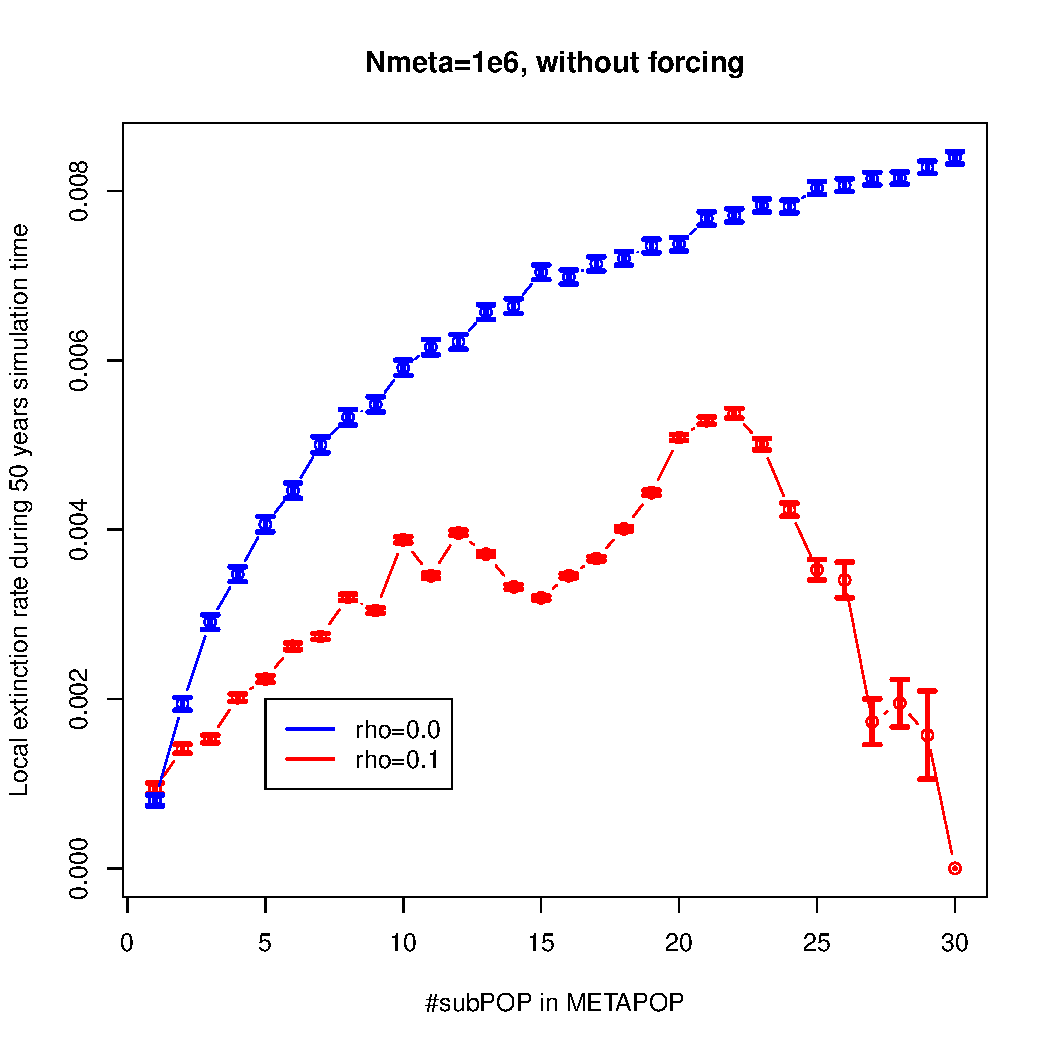
\includegraphics[scale=0.5]{figure/res1METAExtSansForc} 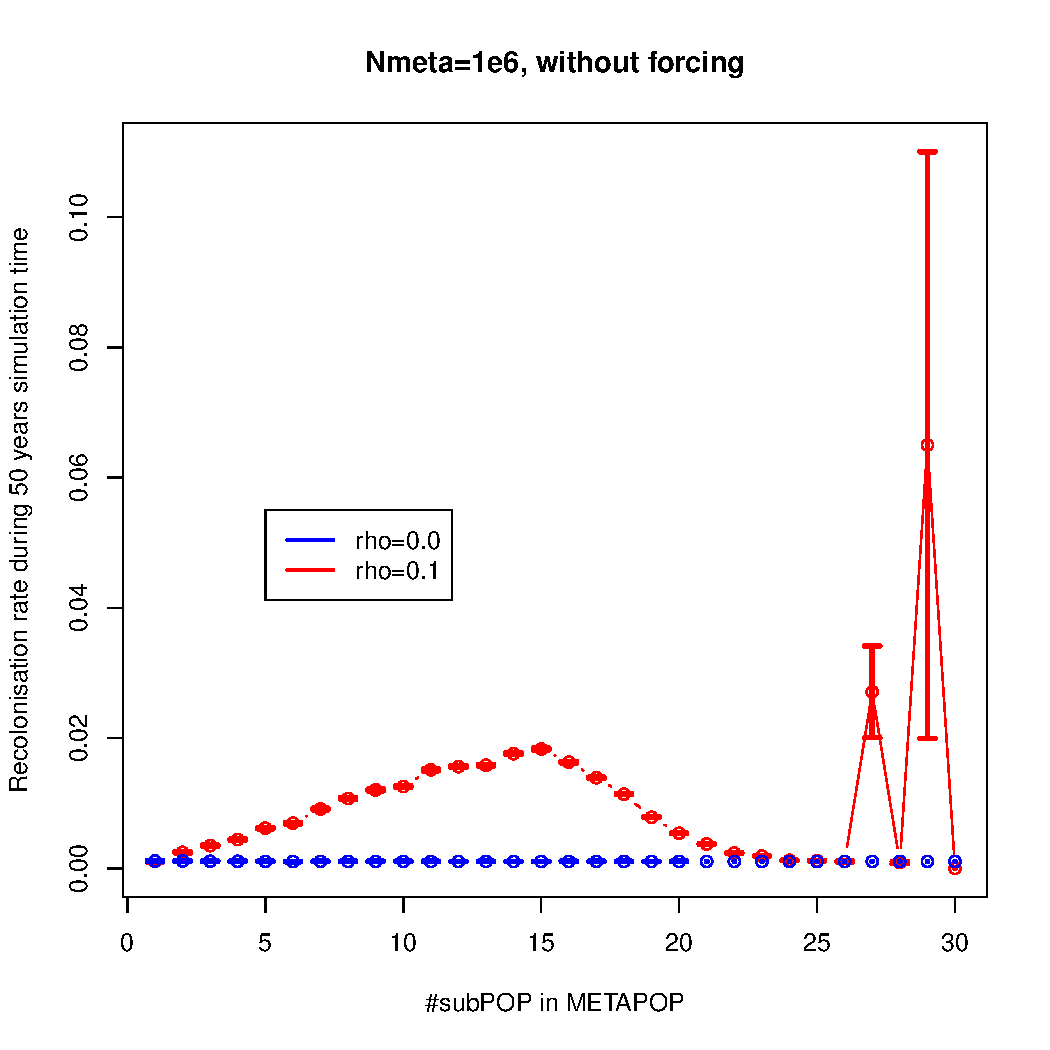
\includegraphics[scale=0.5]{figure/res1METARecolSansForc}\label{figInfNbPOPIslandModel_b}

\label{figInfNbPOPIslandModel_a}

\caption{Influence of the number of subpopulations on the local extinction
rate in the model without the forcing. The number of subpopulations
$n$ from $1$ to $30$, the coupling rate $\rho=0.1$, the fixed
metapopulation size $N=1e6$, the amplitude of season $\kappa_{1}=0$
and $\varphi_{\mbox{\tiny max}}=0$ or $\pi$.}


\label{figInfNbPOPIslandModel}
\end{figure}


In this experience, we are interested in the influence of the number
of subpopulations on the the local extinction rate for the standard
SEIR model without forcing. This simple metapopulation model just
investigates subpopulations connected by individual movement without
environmental transmission. The average number of contacts per unit
of time of a susceptible when visiting another subpopulation is fixed
as a constant. The strength of connection $\rho$ is set to $0$ for
the model of isolated subpopulations (island model) and different
from $0$ for the model of coupled subpopulations (coupling model).
Hence, in this case, the main factor affecting the extinction rate
is the migration of individuals rather any environmental factor. 

The result shown in the Fig \ref{figInfNbPOPIslandModel_a} points
out that in the isolation model with the fixed metapopulation size,
the increased number of subpopulations leads to a decrease of the
subpopulation size. This limits the ability of the rescue effect to
ensure locally extinct subpopulations become recolonized. Hence the
local extinction rate rises significantly. Besides that, due to the
disjunction among subpopulations in the metapopulation, a subpopulation
will obtain the global extinction immediately after it get the first
local extinction, so any there won't be any recolonization occurs
in this island model. The recolonization rate is zero in all cases
as shown in the Fig \ref{figInfNbPOPIslandModel_b}. 

Inverse to the coupled model, the strength of interaction between
the two subpopulations have clearly demonstrated its influence on
the extinction ability in metapopulation. The curve of the coupled
case will be increased notably when the number of subpopulation extends
in the range from $1$ to $20$. As explained in above obtained results
of the Fig \ref{figInflNubPOP}, although the number of subpopulation
augments but is still small, the number of native individuals in a
subpopulation is much larger than the number of tourists in any specific
time. Thus, for the fixed metapopulation size, the increased number
of subpopulations draws a decline of the subpopulation size. The disease
of subpopulation easily get extinct, whenever the local extinction
rate augments. However, when the number of subpopulation becomes a
large number, then the subpopulation size becomes really small, but
the number of neighbours is big. Therefore, the number of native individuals
is much smaller than that of tourists, so the tourists arrive and
continue to transmit disease within the subpopulation. Hence, the
local extinction rate has a significant decline. As pointed out in
the Fig \ref{figInfNbPOPIslandModel_b}, the recolonization rate has
the same form to the local extinction rate. 


\subsection{Influence of the coupling strength on the local extinction rate}

\begin{figure}[h]
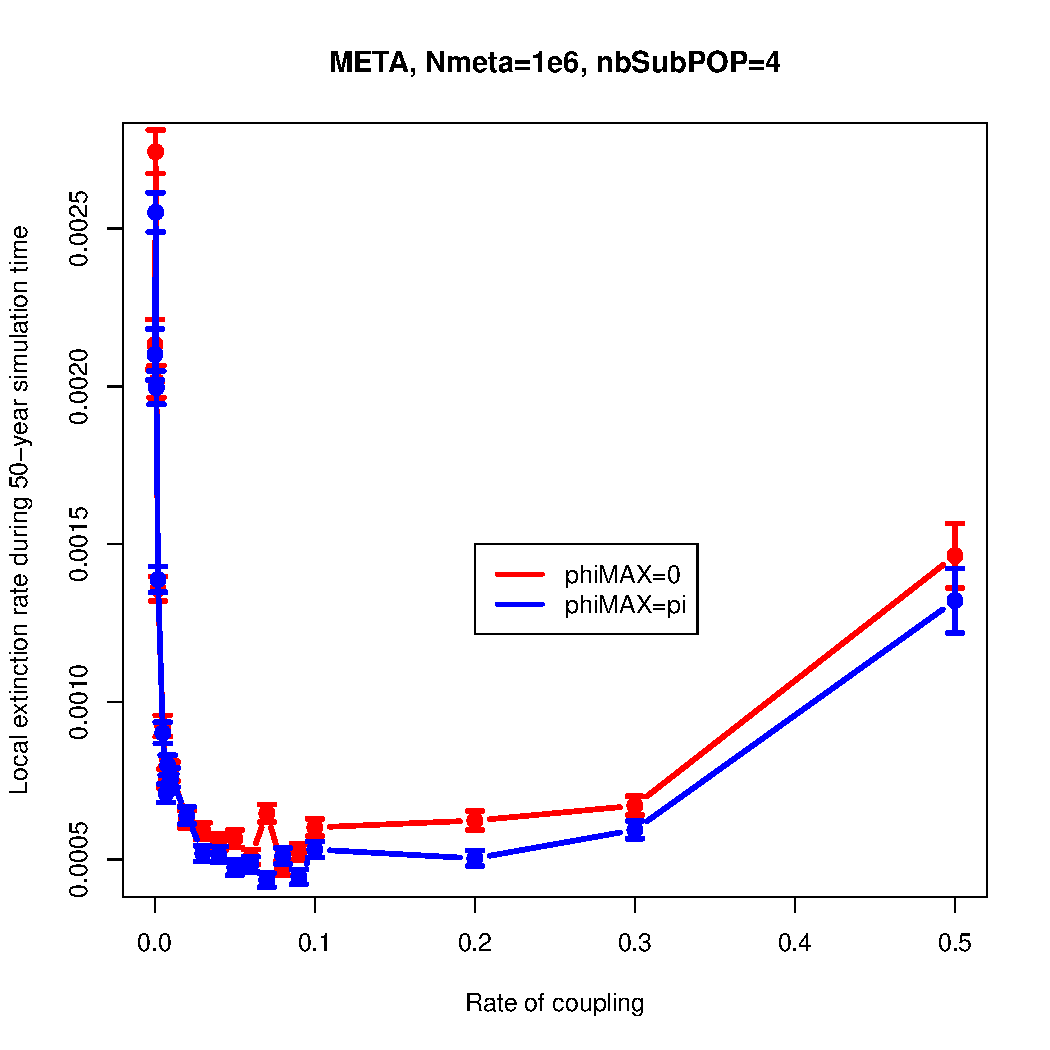
\includegraphics[scale=0.5]{figure/figCoupleMETA}

\caption{Influence of the coupling strength on the local extinction rate of
the metapopulation of 4 subpopulations with the metapopulation size
$N=1e6$}


\label{figCoupleMETA}

\end{figure}


One more factor that was pointed in the introduction part is coupling
strength between subpopulations. Here, the coupling rate or the dispersal
rate $\rho$ can be considered as migration strength. The disease
transmission speed grows fast when coupling rate goes up in metapopulations.
Similar to that, global disease persistence surges also. In this part,
we permit coupling rate change from weak to strong in a metapopulation
of five subpopulations with the population size $N=1e6$ for each
subpopulation. The dispersal rate $\rho$ is divided into three intervals.
These are low, intermediate and high coupling rate intervals. In each
interval, we chose some coupling rates that highlight the coupling
strength among subpopulations in a metapopulation. With each value
of coupling rate, we estimated local extinction rate that presents
the extinction probability of disease in a subpopulation. We have
result as following figure Fig \ref{figCoupleMETA}. 

When the coupling rate is small from $0.0$ to $0.001$, the locale
extinction rate significantly decreases. However, this rate is minimum
when the coupling rate has medium values from$0.001$ to $0.1$. Lastly,
the extinction rate augments back when the coupling rate is very strong
from $0.1$ to $0.5$. As shown in the Fig \ref{figCoupleMETA}, the
local extinction rate in a metapopulation is one humped function for
the coupling rate. The medium coupling rate (from $0.01$ to $0.1$)
minimises the extinction rate of disease in metapopulation. Because
in the case of the small and medium coupling rates, the coupling rate
and the speed of migration among subpopulations are directly proportional.
The dispersal speed increases. Thereby the local recolonization speed
rises, the duration of persistence grows, the local extinction rate
goes down. However, this trend of local extinction with decreasing
coupling rate, is not right any more when the dispersal rate is strong.
The metapopulation has tendency to become one big population. In this
case, the phase difference or the recolonization among subpopulations
are no longer significant. Hence, the local extinction rate rises. 




\section{DISCUSSION}

We successfully have built a version for the susceptible-infected-recovered
stochastic metapopulation model (subpopulations connected by individual
movement), which describes both movement-based and environmental transmission.
The infection rate $\lambda_{i}$ for $subpopulation_{i}$ has portrayed
all effects inside as well as outside of the disease tranmission chain
between individuals in the same subpopulation or in other subpopulations.
Moreover, our metapopulation model became more detailed when we brought
seasonality in metapopulation model to create periodic transmission
in year that highlighted seasonal changes as well as school period
of children \cite{Bolker1993,Bolker1995,Earn1998,Keeling2002}. We
have metapopulation model with different contact rates for each subpopulation.
This is a more complex model than any used metapopulation model. We
have sketched successfully in-phase and sometime out-of-phase (``antiphase'')
models across suburbs of He's 2003 \cite{He2003}.

This complex metapopulation model is also an expected result of Rozhnova(2012)
\cite{Rozhnova2012}. It's a good result for scientists wanting to
use the SEIR metapopulation model for simulating dynamics of infectious
diseases. Our results roughly support those of Rozhnova's 2012. The
authors gave different values of the contact rates $\beta$ of each
subpopulation. However, the rates $\beta$ here are fixed by constants
and the number of subpopulations in experiences are maximum of three.
We don't know why these authors made simulations with just three cities.
We find that, this number of subpopulations is quite small and the
obtained result is not enough strong to ocnfirm. Comparing this result
with our's, in a coupling metapopulation, the degree of synchorny
is maintained when the coupling rate between subpopulations is weak. 

Moreover, our stochastic SEIR metapopulation model with subpopulations
connected to each other, we have quantified disease extinction of
seasonality as well as spatial synchrony. With our model, we can easily
create level of seasonality in year and at the same time, phase difference
in seasonality between subpopulations. It's the reason why we have
model quite close to the metapopulation model in reality.

In addition, for approaches of measuring the probability of disease
persistence in a metapopulation, as previous analyses, the ability
of disease persistence was characterized by fitting an exponential
survival model \cite{Conlan2010,Kleinbaum2005} on a data simulated
by a stochastic model.\textbf{ }To measure the persistence in ecology
and epidemiology, so many methods we can use \cite{Conlan2010,Gunning2013,Keeling2002}.
For example, Keeling et al.(2002) \cite{Keeling2002} gave two methods.
One method was for an isolated metapopulation without migration by
calculating the expected extinction time or the extinction rate during
a given period. This was a theoretical measure as no real data exists
to compare with model results. The other method for a population with
migration was found by calculating the number or the total duration
of extinctions. Then in 2010, ``mean annual fade-out'' and ``fade-outs
post epidemic'' methods proposed by Conlan \cite{Conlan2010} were
used to quantify persistence by basing on the proportion or on the
frequency of zero reports in a given reporting interval. The above
approaches have the same point that they are easily calculated in
all models from simple to complex. But, the obtained results are not
exact, because as we mentionned above, the curves of disease persistence
are Kaplan-Meier survival curves that present the lifetime of every
subpopulation, so the ability of disease persistence is estimated
as a survival function and in fact, it was proved as an exponential
survival model. Hence, in this paper, we have revealed a new method.
We have mesured the rates via Kaplan-Meier survival curves and survival
functions. Our obtained results held the true values of the rates
with the confidence interval of $95\%$.

Due to the phase difference between infection coefficient $\beta$,
we can change by an increase or a decrease in level of synchrony.
We want to decrease level of synchrony, by simply increasing the phase
difference between forcing phase coefficients in the formulas of contact
rate $\beta$. Clearly, the level of synchrony between two subpopulations
are the worst when the two fluctuations are in antiphase (as figure
\ref{figInflNubPOP}). When the phase difference between oscillations
increases, the desynchronizing effect on population dynamics of the
subpopulations augments. This declines the ability of disease extinction.

\begin{figure}
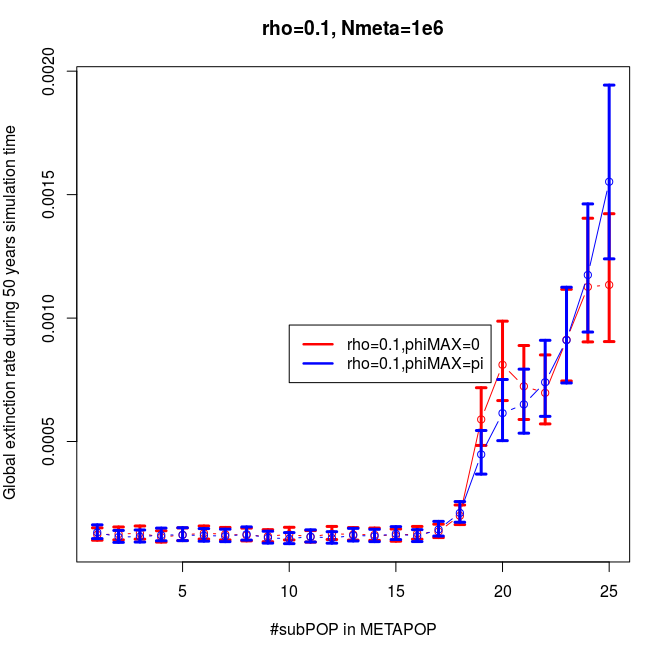
\includegraphics[scale=0.5]{figure/resGlobExt3}

\caption{Quantifing the global extinction rate in the metapopulation. The number
of subpopulation $n$ from $1$ to $25$, the metapopulation size
$N=1e6$ and the coupling rate $\rho=0.1$. As this result, the global
extinction rate of the synchrony with $\varphi_{\mbox{\tiny max}}=0$
has the tendance to be larger than that of the asynchrony with $\varphi_{\mbox{\tiny max}}=\pi$.
Besides, when the number of subpopulation slowly increases from $1$
to $15$, the subpopulation size has a decrease, but this decrease
is very small, the subpopulation size is still very big. Hence, the
red curve of the synchrony and the blue curve of the asynchrony have
a quite near resemblance. Inversely, the global extinction rate strongly
augments when the number of subpopulation is quite big from $20$.
The increased number of subpopulation leads to strongly decline the
subpopulation size. This drives quite the decrease global persitence
time of the metapopualtion, so the mass extinction rate of the metapopulation
increases significantly.}


\label{figMassExt}
\end{figure}


Moreover, as the result above (figure \ref{figInfNbPOPIslandModel})
and the global extinction rate below (figure \ref{figMassExt}), our
results, along with those of Bolker (1995) \cite{Bolker1995} and
Heino (1997) \cite{Heino1997}, stress the local extinction rate being
inversely proportionnel with the global extinction rate in a metapopulation.
When the level of synchrony is at a reduction and the global persistence
time gets an increase, the global extinction rate of metapopulation
goes down and the local extinction rate goes up. Due to the result
about local extinction, we also affirm that disease is always available
in metapopulation if and only if at least one subpopulaiton is not
extinct. 

Our finding has specified the two main factors influencing the persistence
ability of an infectious disease. One factor is transmission characteristics
of the infectious disease and the other is interplay between mixing
subpopulations in metapopulation. The interaction between the disease
persistence and the spatial heterogeneity becomes a major key to unlock
questions about infectious disease in epidemiology. This result takes
a large part in epidemic disease persistence domain that has being
exploited in scientific epidemically research works. We gained a robust
understanding of how disease extinction is affected by local factors
such as spatial heterogeneity, demographic asynchrony and seasonality,
as well as mixing factors such as migration, disease transmission
between hosts and pathogens. Lastly, we also highlighted recolonization
effects. It is like rescue for disease. Because of connection between
subpopulation, individuals can go everywhere. Subpopulation is quickly
re-infected althought the disease has became extinct. Thus, the disease
rescus makes local extintions difficult to extend into global extinctions.

As a matter of the fact of coupling strength among subpopulations
in metapopulation, we proved that\textbf{ }the extinction of the disease
in the metapopulation is not only computed by a exponential survival
function over time, but also a concave function for the coupling rate.
In addition, the disease extinction in metapopulation is minimum when
the coupling rate between subpopulations is just medium. This finding
is similar to those of Huffaker(1958) \cite{huffaker1958experimental},
Holyoak and Lawler(1996) \cite{holyoak1996persistence}, and Yaari
et al. (2012) \cite{Yaari2012} when they exhaustively explored the
disease persistence behavior of many different metapopulation models.
And our result one more time affirms that the disease persistence
and the interaction in metapopulation models are significant when\textbf{
}the interaction strength $\rho$ is from $10^{-3}$ to 0.1 \cite{KeelingRohani2008}.

To summarize, we have built successfully a\textbf{ }sinusoidally forced
SEIR stochastic metapopulation model. This model is like a physical
system of coupled oscillators. We have pointed out that spatial synchronization
consistently and predictably makes extinction risk increase by using
the model $0$ where all the subpopulations have the same population
size $N$ and there is no explicit spatial distance. So, it's good
for the future, we can continue this work with different population
size of each subpopulation and different spatial distance between
subpopulations and then, create synchronous metapopulations that optimize
vaccination policies.

\bibliographystyle{plain}
\bibliography{bib/bikBokEpidemics,bib/bikCCS,bib/bikPerSyns}



\section{Appendix : equilibrium values of the system \ref{eq:dS}--\ref{eq:dR}}

We start with ordinary differential equations for a $subpopulation_{i}$
in a metapopulation as follows:

\begin{eqnarray}
\frac{dS_{i}}{dt} & = & \mu N_{i}-\lambda_{i}S_{i}-\mu S_{i}\\
\frac{dE_{i}}{dt} & = & \lambda_{i}S_{i}-\mu E_{i}-\sigma E_{i}\\
\frac{dI_{i}}{dt} & = & \sigma E_{i}-\mu I_{i}-\gamma I_{i}\\
\frac{dR_{i}}{dt} & = & \gamma I_{i}-\mu R_{i}
\end{eqnarray}
 In simulation, we know that the equilibrium state allow a disease
to persist in a population for a long time. So, an infectious disease
in the $subpopulation_{i}$ is available in long term this system
is at equilibrium. It means that at which $\frac{dS_{i}}{dt}=\frac{dE_{i}}{dt}=\frac{dI{}_{i}}{dt}=\frac{dR{}_{i}}{dt}=0$
({*}). Thus, we let all equations (equations $15$ - $18$ ) in the
system be equal to zero, then calculate the values of the variables
(now denoted by $S_{i}^{*}$, $E_{i}^{*}$, $I_{i}^{*}$ , and $R{}_{i}^{*}$)
that satisfy this condition ({*}). We have these values as folllows:

\begin{eqnarray}
S_{i}^{*} & = & N_{i}\frac{(\gamma+\mu)(\sigma+\mu)}{\beta\sigma}\\
E_{i}^{*} & = & N_{i}\mu\left(\frac{1}{\sigma+\mu}-\frac{\gamma+\mu}{\beta\sigma}\right)\\
I_{i}^{*} & = & N_{i}\mu\frac{\beta\sigma-(\sigma+\mu)(\gamma+\mu)}{\beta(\sigma+\mu)(\gamma+\mu)}\\
R_{i}^{*} & = & N_{i}-S_{i}^{*}-E_{i}^{*}-I_{i}^{*}
\end{eqnarray}


Here, if we set $R_{0}=\frac{\beta\sigma}{(\gamma+\mu)(\sigma+\mu)}$,
so we have

\begin{eqnarray}
S_{i}^{*} & = & N_{i}\frac{1}{R_{0}}\\
E_{i}^{*} & = & N_{i}\frac{\mu\sigma}{R_{0}}\left(R_{0}-1\right)\\
I_{i}^{*} & = & N_{i}\frac{\mu}{\beta}(R_{0}-1)\\
R_{i}^{*} & = & N_{i}-S_{i}^{*}-E_{i}^{*}-I_{i}^{*}
\end{eqnarray}


One nomal conditions for all population availabes is that the equilibrium
values cannot be negative. Therefore, an infectious disease is available
in the $subpopulation_{i}$ if $R_{0}>1$. Now, the endemic equilibrium
in the system is given by $(S_{i}^{*},E_{i}^{*},I{}_{i}^{*},R{}_{i}^{*})$
= $(N_{i}\frac{1}{R_{0}}$, $N_{i}\frac{\mu\sigma}{R_{0}}\left(R_{0}-1\right)$,
$N_{i}\frac{\mu}{\beta}(R_{0}-1)$, $N_{i}(1-\frac{1}{R_{0}}-\frac{\mu\sigma}{R_{0}}\left(R_{0}-1\right)-\frac{\mu}{\beta}(R_{0}-1))$.


\subsection{Stationary distribution in metapopulation}

Here we show some assumptions for the stationary distribution model
as follows :
\begin{itemize}
\item Assumption 1. For each city $V_{i}$, there exists a markov chain
$M_{i}$ describing where (i.e. in which city) individuals native
from $V_{i}$ travel at each time step. 
\item Assumption 2. Each $M_{i}$ has a stationary distribution $\rho(M_{i})$. 
\item Assumption 3. At time t=0, each agent is located in a city randomly
drawn from $\rho(M_{i})$.
\end{itemize}
When we consider a simplified model in which the dynamics of the agents
is stationary: each agent native from $V_{i}$ no more follows a markov
chain, but is relocated at each time step on a city randomly drawn
from $\rho(M_{i})$.

Then, under assumptions 1,2,3, at any time $t$, when the total number
of agents grows to infinity, the size of the populations under the
markovian dynamics converges towards the size of the populations under
stationary dynamics.

Hence, any statistics computed on the densities of agents from the
same population in various cities will not distinguish the markovian
from the stationary dynamics. 

Based on this conclusion, we will deploy a stationary distribution
in a metapopulation. First of all, we choose a population size N for
the metapopulation. Then, we compute the After that, the transition
matrix converge towards a stationary distribution matrix. Finally,
we apply the stationary distribution matrix in the metapopulation
of n subpopulations


\section{Appendix: derivation of the equation \ref{eq:force-1}}

Here, we will point out that the contact rate $\beta$ is a function
of the average contact number per unit of time and the probability
of successful disease transmission following a contact.
\begin{defn}
During the small time interval $\delta t$, each individual native
of the city $i$ visits one single city\textbf{ }$j$ (with the probability
$\rho_{ij}$) and will see in average $\kappa_{j}$ individuals. These
individuals come from all the cities.
\end{defn}

\subsection{Notation :}

Here, we present list of sets and events describing the state of the
system at time $t$ : 
\begin{itemize}
\item $C_{i}$ is the set of all individuals born in subpopulation $i$. 
\item $V_{i,t}$ is the set of all individuals physically located in subpopulation
$i$ from time $t$ to time $t+\delta t$. This includes foreigners
traveling in subpopulation $i$ at time $t$, and all natives from
subpopulation $i$ which are not traveling abroad at time $t$. 
\item $S_{t},E_{t},I_{t},R_{t}$ are the sets of all individuals respectively
susceptible, exposed, infected and recovered at time $t$. Note that
these set include individuals from all subpopulations. 
\item $S_{i,t},E_{i,t},I_{i,t},R_{i,t}$ are the same sets, restricted to
natives of subpopulation $i$. So formally, $S_{i,t}=S_{t}\cap C_{i}$,
$E_{i,t}=E_{t}\cap C_{i}$, $I_{i,t}=I_{t}\cap C_{i}$, and $R_{i,t}=R_{t}\cap C_{i}$. 
\item $Transmit(y,x)$ is an event indicating that individual $x$ gets
infected by individual $y$ which was already infected 
\item $c_{i,k}$ is the probability that a susceptible individual native
from $i$ being in contact with another infected individual native
from $k$ gets infected. 
\item $\kappa_{j}$ is the average number of contacts per unit of time a
susceptible will have when visiting city $j$. 
\item $\xi_{jk}$ refers to the probability that an individual $y$ meeting
$x$ in $C_{j}$ comes from $C_{k}$.
\item $\rho_{i,j}$, the probability that an individual from subpopulation
$i$ visits subpopulation $j$. Of course, $\sum_{j=1}^{M}\rho_{ij}=1$.\end{itemize}
\begin{prop}
The coefficient $\kappa$ should also depend on $i$, because an individual
native from city $i$ meets more people in his own city than abroad
($\kappa_{i,i}>\kappa_{i,j}$). 
\end{prop}

\subsection{The background}

One general question is always posed ``how does the population of
exposed individuals of subpopulation $i$ evolve ?''. For the sake
of simplicity, in the process of transmission of the SEIR model, we
focus on the incidence and we assume for now that the latent period
and the recovery rate, repectively $\mu=\sigma=0$. Thus, we write
a probabilistic formulation of $\frac{dE_{i}}{dt}$. Assuming the
time is discrete, we have $\frac{dE_{i}}{dt}\approx\mathbb{E}\left[E_{i,t+1}\setminus E_{i,t}\right]$.
Then,

\begin{eqnarray*}
\mathbb{E}\left[E_{i,t+1}\setminus E_{i,t}\right] & = & \mathbb{E}\left[E_{i,t+1}\cap S_{i,t}\right]\\
 & = & \sum_{x\in C_{i}}Pr\left[x\in E_{t+1}\wedge x\in S_{t}\right]\\
 & = & \sum_{x\in C_{i}}Pr\left[x\in S_{t}\right]*Pr\left[x\in E_{t+1}\mid x\in S_{t}\right]\\
 & = & Pr_{x\sim\mathcal{X}_{i}}\left[x\in E_{t+1}\mid x\in S_{t}\right]*\sum_{x\in C_{i}}Pr\left[x\in S_{t}\right]\\
 & = & |S_{i,t}|\times Pr_{x\sim\mathcal{X}_{i}}\left[x\in E_{t+1}\mid x\in S_{t}\right]
\end{eqnarray*}


Assume there are $M$ cities. An individual $x$ of the subpopulation
$i$ may be visiting another subpopulation, or staying in its own
subpopulation. Applying the law of total probabilities, we get:

\begin{eqnarray*}
Pr_{x\sim\mathcal{X}_{i}}\left[x\in E_{t+dt}\mid x\in S_{t}\right] & = & \sum_{j=1}^{M}Pr_{x\sim\mathcal{X}_{i}}\left[x\in E_{t+dt}\wedge x\in V_{j,t}\mid x\in S_{t}\right]\\
 & = & \sum_{j=1}^{M}Pr_{x\sim\mathcal{X}_{i}}\left[x\in E_{t+dt}\mid x\in S_{t}\wedge x\in V_{j,t}\right].Pr_{x\sim\mathcal{X}_{i}}\left[x\in V_{j,t}\right]\\
 &  & \sum_{j=1}^{M}Pr_{x\sim\mathcal{X}_{i}}\left[x\in E_{t+dt}\mid x\in S_{t}\wedge x\in V_{j,t}\right]\times\rho_{ij}
\end{eqnarray*}


Where $\rho_{i,j}=Pr_{x\sim\mathcal{X}_{i}}\left[x\in V_{j,t}\right]$,
the probability that an individual from subpopulation $i$ visits
subpopulation $j$. Of course, $\sum_{j=1}^{M}\rho_{ij}=1$.


\subsection{Study of case where agent $x$ native from city $i$ visits city
$j$}

Here, we look at the probability that a susceptible $x\sim\mathcal{X}_{i}$
visiting $j$ gets infected or not after $\delta t$ time steps. Let
$\mathcal{Y}$ be the uniform distribution over $V_{j,t}$. The correct
mathematical approach for this would be to assume that for each city
$k$, the number of people native from $k$ that we meet during $\delta t$
follows a Poisson process. So both the number of people we meet and
the number of infected people we meet during $\delta t$ should be
random variables.

In the approach described in \cite{KeelingRohani2008}, the authors
did not do this. They assumed that both the number of people we meet
and the number of infected people we meet \emph{are fixed} (otherwise
the maths they write would have been different). We will call this
the ``Keeling \& Rohani'' interpretation that we will present it
in the following parts.

We introduce an alternative approximation, where we assume that the
number $\kappa$ of people we meet during $\delta t$ is \emph{fixed},
but each of these people has \emph{some probability} to be infected.
This is an \emph{in-between interpretation}, easier than the Poisson
process maths, but better than Keeling\&Rohani's one. We will call
this the ``Yann-Giang'' interpretation.


\subsubsection{The ``Yann-Giang'' interpretation}
\begin{prop}
Agent $x$ meets \emph{exactly} $\kappa_{j}$ other individuals, and
each of these individuals has a probability $\frac{\left|I_{k,t}\right|}{N_{k}}$
of being infected, where $k$ is its native city. Let $y_{1}\ldots y_{\kappa_{j}}$
be the individuals that $x$ meets. We get:
\end{prop}
\begin{eqnarray*}
 &  & Pr_{x\sim\mathcal{X}_{i}}\left[x\in S_{t+\delta t}\mid x\in S_{t}\wedge x\in V_{j,t}\right]\\
 & = & Pr_{x\sim\mathcal{X}_{i},y_{1}\ldots,y_{\kappa_{j}}\sim\mathcal{Y}}\left[\bigwedge_{p=1}^{\kappa_{j}}\neg\left(y_{p}\in I_{t}\wedge Transmit(y_{p},x)\right)\mid x\in S_{t}\wedge x\in V_{j,t}\right]
\end{eqnarray*}


So we have:

\begin{eqnarray*}
 &  & Pr_{x\sim\mathcal{X}_{i}}\left[x\in S_{t+\delta t}\mid x\in S_{t}\wedge x\in V_{j,t}\right]\\
 & = & Pr_{x\sim\mathcal{X}_{i},y\sim\mathcal{Y}}\left[\neg\left(y\in I_{t}\wedge Transmit(y,x)\right)\mid x\in S_{t}\wedge x\in V_{j,t}\right]^{\kappa_{j}\delta t}
\end{eqnarray*}


Moreover, we have:
\begin{itemize}
\item the probability so that a susceptible individual $x$ is infected
by an infected individual $y$ :
\end{itemize}
\begin{eqnarray*}
 &  & Pr_{x\sim\mathcal{X}_{i},y\sim\mathcal{Y}}\left[y\in I_{t}\wedge Transmit(y,x)\mid x\in S_{t}\wedge x\in V_{j,t}\right]\\
 & = & \sum_{k=1}^{M}Pr_{x\sim\mathcal{X}_{i},y\sim\mathcal{Y}}\left[y\in I_{t}\wedge Transmit(y,x)\mid x\in S_{t}\wedge x\in V_{j,t}\wedge y\in C_{k}\right].Pr_{y\sim\mathcal{Y}}\left(y\in C_{k}\right)\\
 & = & \sum_{k=1}^{M}\left\{ Pr_{x\sim\mathcal{X}_{i},y\sim\mathcal{X}_{k}}\left[y\in I_{t}\mid x\in S_{t}\wedge x\in V_{j,t}\right]\right.\\
 &  & \,\,\,\,\,\left.\times Pr_{x\sim\mathcal{X}_{i},y\sim\mathcal{X}_{k}}\left[Transmit(y,x)\mid y\in I_{t}\wedge x\in S_{t}\wedge x\in V_{j,t}\wedge y\in C_{k}\right]\times Pr_{y\sim\mathcal{Y}}\left(y\in C_{k}\right)\right\} \\
 & = & \sum_{k=1}^{M}\left(\frac{\left|I_{k,t}\right|}{N_{k}}\times c_{ik}\times\xi_{jk}\right)
\end{eqnarray*}


$\xi_{jk}=\frac{N_{k}\rho_{kj}}{\sum_{v=1}^{M}N_{v}\rho_{vj}}$ refers
to the probability that an individual $y$ meeting $x$ in $C_{j}$
comes from $C_{k}$.
\begin{itemize}
\item hence, the probability so that a susceptible individual $x$ is not
infected by an infected individual $y$ :
\end{itemize}
\[
1-\sum_{k=1}^{M}\left(\frac{\left|I_{k,t}\right|}{N_{k}}\times c_{ik}\times\xi_{jk}\right)
\]

\begin{itemize}
\item thereby, the probability so that a susceptible individual $x$ is
not infected after $\kappa_{j}$ contacts per unit time $\delta t$.
\end{itemize}
\[
\left[1-\sum_{k=1}^{M}\left(\frac{\left|I_{k,t}\right|}{N_{k}}\times c_{ik}\times\xi_{jk}\right)\right]^{\kappa_{j}\delta t}
\]

\begin{itemize}
\item thus, the probability so that a susceptible individual $x$ becomes
infected after $\kappa_{j}$ contacts per unit time $\delta t$.
\end{itemize}
\begin{eqnarray*}
Pr_{x\sim\mathcal{X}_{i}}\left[x\in E_{t+\delta t}\mid x\in S_{t}\wedge x\in V_{j,t}\right] & = & \left[1-\sum_{k=1}^{M}\left(\frac{\left|I_{k,t}\right|}{N_{k}}\times c_{ik}\times\xi_{jk}\right)\right]^{\kappa_{j}\delta t}
\end{eqnarray*}


We now apply the \emph{log} approximation which consists in approximating
$1-(1-u)^{v}$ by $v\log(1-u)$:

\begin{eqnarray*}
Pr_{x\sim\mathcal{X}_{i}}\left[x\in E_{t+\delta t}\mid x\in S_{t}\wedge x\in V_{j,t}\right] & = & -\kappa_{j}\delta t\log\left[1-\sum_{k=1}^{M}\left(\frac{\left|I_{k,t}\right|}{N_{k}}\times c_{ik}\times\xi_{jk}\right)\right]
\end{eqnarray*}


So, the transmission rate per susceptible individual is as follows
:

\[
\frac{dPr_{x\sim\mathcal{X}_{i}}\left[x\in E_{t+dt}\mid x\in S_{t}\wedge x\in V_{j,t}\right]}{dt}\simeq-\kappa_{j}\log\left[1-\sum_{k=1}^{M}\left(\frac{\left|I_{k,t}\right|}{N_{k}}\times c_{ik}\times\xi_{jk}\right)\right]
\]


In fact, we use the parameter $\lambda$ to present this quantity,
and it is denoted as the ``force of infection'' :

\[
\lambda_{i}=\sum_{j}\rho_{ij}\kappa_{j}\log\left[1-\sum_{k=1}^{M}\left(\frac{\left|I_{k,t}\right|}{N_{k}}\times c_{ik}\times\xi_{jk}\right)\right]
\]


If there is only one city $i$, then

\[
\lambda_{i}=\kappa_{j}log(1-\frac{\left|I_{i}\right|}{N_{i}}\times c_{ii})
\]



\subsubsection{``Keeling \& Rohani'' Interpretation}
\begin{prop}
Agent $x$ meets \emph{exactly} $\kappa_{j}\delta t\xi_{jk}\frac{\left|I_{k,t}\right|}{N_{k}}$
other infected individuals native from city $k$.

Let $l_{k}=\kappa_{j}\delta t\xi_{jk}\frac{\left|I_{k,t}\right|}{N_{k}}$. 


Let $y_{1}^{k}\ldots y_{l_{k}}^{k}$ be the infected individuals native
from $k$ that our individual $x$ meets between $t$ and $t+\delta t$.

\end{prop}
We have the probability so that a susceptible individual $x$ is not
infected after having seen $l_{k}$ individuals between $t$ and $t+\delta t$
:

\begin{eqnarray*}
 &  & Pr_{x\sim\mathcal{X}_{i}}\left[x\in S_{t+\delta t}\mid x\in S_{t}\wedge x\in V_{j,t}\right]\\
 & = & Pr_{x\sim\mathcal{X}_{i}}\left[\bigwedge_{\begin{array}{c}
k=1\ldots M\\
p=1\ldots l_{k}
\end{array}}\neg\left(Transmit(y_{p}^{k},x)\right)\mid x\in S_{t}\wedge x\in V_{j,t}\right]\\
 & = & \prod_{k=1}^{M}Pr_{x\sim\mathcal{X}_{i}}\left[\bigwedge_{p=1\ldots l_{k}}\neg\left(Transmit(y_{p}^{k},x)\right)\mid x\in S_{t}\wedge x\in V_{j,t}\right]\\
 & = & \prod_{k=1}^{M}\left(1-c_{ik}\right)^{\kappa_{j}\delta t\xi_{jk}\frac{\left|I_{k,t}\right|}{N_{k}}}
\end{eqnarray*}


Then, we plug this back into the previous formula, and we get:

\begin{eqnarray*}
Pr_{x\sim\mathcal{X}_{i}}\left[x\in E_{t+\delta t}\mid x\in S_{t}\wedge x\in V_{j,t}\right] & = & 1-\prod_{k=1}^{M}\left(1-c_{ik}\right)^{\kappa_{j}\xi_{jk}\frac{\left|I_{k,t}\right|}{N_{k}}\delta t}
\end{eqnarray*}


The first order approximation of $1-\prod_{k=1}^{M}(1-c_{ik})^{v_{k}}$
is $\sum_{k=1}^{M}-v_{k}\log(1-c_{ik})$. Applying this approximation
here, we get:

\begin{eqnarray*}
Pr_{x\sim\mathcal{X}_{i}}\left[x\in E_{t+\delta t}\mid x\in S_{t}\wedge x\in V_{j,t}\right] & \simeq & \delta t\sum_{k=1}^{M}\left(-\kappa_{j}\xi_{jk}\frac{\left|I_{k,t}\right|}{N_{k}}\log\left(1-c_{ik}\right)\right)
\end{eqnarray*}


Define $\beta_{ijk}=-\kappa_{j}\log\left(1-c_{ik}\right)$, let $\delta t$
converge to zero, and we get:

\[
\frac{dPr_{x\sim\mathcal{X}_{i}}\left[x\in E_{t+dt}\mid x\in S_{t}\wedge x\in V_{j,t}\right]}{dt}\simeq\sum_{k=1}^{M}\left(\xi_{jk}\frac{\left|I_{k,t}\right|}{N_{k}}\beta_{ijk}\right)
\]


If there is only one city $i$, then we fall back to the formula of
\cite{KeelingRohani2008}. We have : 

\[
\beta_{i}=-\kappa_{i}\log\left(1-c_{i}\right)
\]


\[
\frac{d}{dt}\mathbb{E}\left[\left|E_{i,t+dt}-E_{i,t}\right|\right]\simeq-\left|S_{i,t}\right|\left(\frac{\left|I_{i}\right|}{N_{i}}\beta_{i}\right)
\]


and the force of infection as follows :

\[
\lambda_{i}=\beta_{i}\frac{\left|I_{i}\right|}{N_{i}}
\]



\subsection{Final Formula}

We simply have to plug in the probability $\rho_{ij}$ that $i$ visits
$j$.

We get, for the ``Yann-Giang'' interpretation :

\[
\frac{d}{dt}\mathbb{E}\left[\left|E_{i,t+dt}-E_{i,t}\right|\right]\simeq-\left|S_{i,t}\right|\sum_{j}\rho_{ij}\kappa_{j}\log\left[1-\sum_{k=1}^{M}\left(\frac{\left|I_{k,t}\right|}{N_{k}}\times c_{ik}\times\xi_{jk}\right)\right]
\]


And for the ``Keeling \& Rohani'' Interpretation :

\[
\frac{d}{dt}\mathbb{E}\left[\left|E_{i,t+dt}-E_{i,t}\right|\right]\simeq-\left|S_{i,t}\right|\sum_{j}\rho_{ij}\sum_{k=1}^{M}\left(\xi_{jk}\frac{\left|I_{k,t}\right|}{N_{k}}\beta_{ijk}\right)
\]



\section{Appendix : Characterization of synchrony}

Call $\delta_{ij}=\delta_{ji}$ ($0\leqslant\delta_{ij}<2\pi$) the
phase difference between subpopulations $i$ and $j$ : 
\begin{equation}
\delta_{ij}=|\varphi_{i}-\varphi_{j}|\bmod2\pi
\end{equation}
 where $\varphi{}_{i}$ and $\varphi{}_{j}$ are the phases of the
contact rates (equation \ref{eq:beta_i}) in subpopulations $i$ et
$j$. Populations $i$ and $j$ are perfectly in phase if $\delta_{ij}=\delta_{ji}=0$
or $2\pi$ and in opposition of phase if $\delta_{ij}=\delta_{ji}=\pi$.
We can thus define the degree of synchrony $\xi_{ij}=\xi_{ji}$ ($0\leqslant\xi_{ij}\leqslant1$)
between populations $i$ and $j$ as 
\begin{equation}
\xi_{ij}=1-\frac{\left|\delta_{ij}\right|}{\pi}.
\end{equation}
 
\begin{figure}[htpb]
\centering 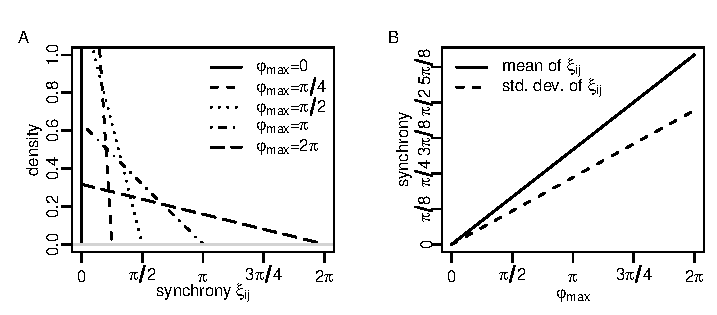
\includegraphics{figure/figure1} \caption{\label{fig:synchrony-1}Synchrony in the case of model 0. (A) distribution
of synchrony $\xi_{ij}$ for various values of $\varphi_{max}$. (B)
mean and standard deviation of the distribution of $\xi_{ij}$ as
functions of $\varphi_{\mbox{\tiny max}}$.}
\end{figure}


Consider that in the metapopulation the phases $\varphi_{i}$ of the
contact rates in the $n$ subpopulations are evenly distributed between
0 and $\varphi_{\mbox{\tiny max}}$ ($0\leqslant\varphi_{\mbox{\tiny max}}\leqslant\pi$).
We can express the mean of the pairwise phase differences $\delta_{ij}=\delta_{ji}$
as 
\begin{equation}
<\!\!\delta_{ij}\!\!>\;=\;<\!\!\delta_{ji}\!\!>\;=2\varphi_{\mbox{\tiny max}}\sum_{k=1}^{n-1}\frac{(n-k)k}{(n-1)n^{2}}=\frac{n+1}{3n}\varphi_{\mbox{\tiny max}}
\end{equation}
 and thus the mean of the synchronies $\xi_{ij}=\xi_{ji}$ as 
\begin{equation}
<\!\!\xi_{ij}\!\!>\;=\;<\!\!\xi_{ji}\!\!>\;=1-\frac{n+1}{3n}\frac{\varphi_{\mbox{\tiny max}}}{\pi}
\end{equation}
 and thus 
\begin{equation}
\lim_{n\to\infty}<\!\!\xi_{ij}\!\!>\;=1-\frac{\varphi_{\mbox{\tiny max}}}{3\pi}
\end{equation}


This last result shows that, for a high enough number $n$ of subpopulations,
the mean value of the $\xi_{ij}$ does not depend on the number of
subpopulation.

The values of $\varphi_{i}$ are chosen so that they are uniformly
distributed between $\varphi_{\mbox{\tiny min}}=0$ and $\varphi_{\mbox{\tiny max}}$.
The distribution of $\xi_{ij}$ doesn't depend on $n$ the number
of subpopulation, but only depends $\varphi_{\mbox{\tiny max}}$ and
may be is characterized by one single parameter (we choose the average
value of all $\xi_{ij}$), view figure \ref{fig:synchrony-1}.

------
\end{document}
